% !TEX program = pdflatex
\documentclass[aspectratio=169]{beamer}
\usetheme{Madrid}
\usecolortheme{default}
\usepackage{tikz}

% Custom colors
\definecolor{myblue}{RGB}{0,114,178}
\definecolor{myorange}{RGB}{230,159,0}
\definecolor{mygreen}{RGB}{0,158,115}
\definecolor{myred}{RGB}{213,94,0}
\definecolor{mypurple}{RGB}{204,121,167}
\definecolor{mybrown}{RGB}{240,228,66}
\definecolor{mygray}{RGB}{189,189,189}

% Set colors
\setbeamercolor{title}{fg=white,bg=myblue}
\setbeamercolor{frametitle}{fg=white,bg=myblue}
\setbeamercolor{section title}{fg=white,bg=myblue}
\setbeamercolor{subsection title}{fg=white,bg=myorange}
\setbeamercolor{item}{fg=myblue}
\setbeamercolor{subitem}{fg=myorange}

% Remove navigation symbols
\setbeamertemplate{navigation symbols}{}

% Title page
\title{Linear Approximation \& Taylor Polynomials}
\subtitle{Applications of Derivatives: Approximating Functions}
\author{Differential Calculus}
\date{}

\begin{document}

\begin{frame}
\titlepage
\end{frame}

\begin{frame}{Outline}
\tableofcontents
\end{frame}

\section{Introduction}

\begin{frame}{Why Linear Approximation?}
\begin{itemize}
    \item Sometimes we need to approximate function values that are difficult to compute exactly
    \item Linear approximation uses the tangent line to estimate function values near a known point
    \item It's based on the idea that near a point, a function looks approximately linear
    \item Applications include:
    \begin{itemize}
        \item Estimating square roots, exponentials, logarithms
        \item Error analysis in measurements
        \item Quick mental calculations
        \item Understanding function behavior locally
    \end{itemize}
\end{itemize}
\end{frame}

\section{Zeroth Approximation}

\begin{frame}{Zeroth Approximation}
\begin{itemize}
    \item The simplest approximation: use a constant function
    \item $F(x) = f(a)$ for all $x$
    \item This is just the function value at the point $a$
    \item Very crude approximation - only good at the point itself
    \item Example: $f(x) = e^x$ at $a = 0$ gives $F(x) = 1$
\end{itemize}
\end{frame}

\section{First Approximation - Linear Approximation}

\begin{frame}{Linear Approximation Concept}
\begin{itemize}
    \item Improve on zeroth approximation by using a linear function
    \item Allow $F(x) = A + Bx$ for some constants $A$ and $B$
    \item Requirements:
    \begin{itemize}
        \item $F(a) = f(a)$ (same value at $x = a$)
        \item $F'(a) = f'(a)$ (same slope at $x = a$)
    \end{itemize}
    \item This means $F(x)$ is the tangent line to $f(x)$ at $x = a$
\end{itemize}
\end{frame}

\begin{frame}{Deriving the Linear Approximation}
\textbf{Step-by-step derivation:}
\begin{itemize}
    \item Let $F(x) = A + Bx$
    \item Then $F(a) = A + Ba = f(a)$
    \item And $F'(x) = B$, so $F'(a) = B = f'(a)$
    \item Therefore $B = f'(a)$
    \item Substitute: $A + a \cdot f'(a) = f(a)$
    \item So $A = f(a) - a \cdot f'(a)$
\end{itemize}
\end{frame}

\begin{frame}{Linear Approximation Formula}
\textbf{The Linear Approximation:}
\[f(x) \approx f(a) + f'(a)(x - a)\]

\textbf{Key Points:}
\begin{itemize}
    \item This is exactly the equation of the tangent line at $x = a$
    \item Good approximation for $x$ close to $a$
    \item Requires knowing $f(a)$ and $f'(a)$
    \item The approximation improves as $x$ gets closer to $a$
\end{itemize}
\end{frame}

\begin{frame}{Geometric Interpretation}
\begin{center}
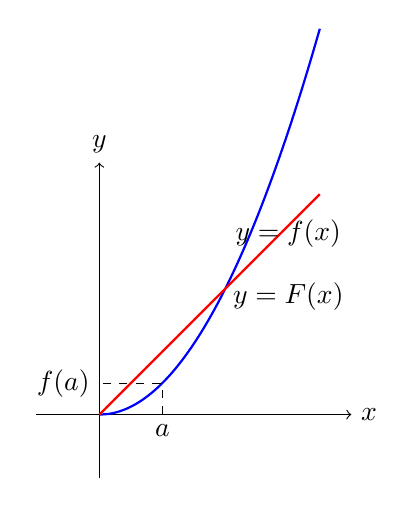
\begin{tikzpicture}[scale=0.8]
\draw[->] (-1,0) -- (4,0) node[right] {$x$};
\draw[->] (0,-1) -- (0,4) node[above] {$y$};
\draw[domain=0:3.5, smooth, variable=\x, blue, thick] plot ({\x}, {0.5*\x*\x});
\draw[domain=0:3.5, smooth, variable=\x, red, thick] plot ({\x}, {1 + 1*(\x-1)});
\draw[dashed] (1,0) -- (1,0.5) -- (0,0.5);
\node[below] at (1,0) {$a$};
\node[left] at (0,0.5) {$f(a)$};
\node[above] at (3,2.5) {$y = f(x)$};
\node[above] at (3,1.5) {$y = F(x)$};
\end{tikzpicture}
\end{center}

\textbf{Visual:}
\begin{itemize}
    \item Blue curve: $y = f(x)$
    \item Red line: $y = F(x)$ (tangent line)
    \item The tangent line stays close to the curve near $x = a$
\end{itemize}
\end{frame}

\section{Examples}

\begin{frame}{Example 1: Estimating $e^{0.1}$}
\textbf{Problem:} Use linear approximation to estimate $e^{0.1}$

\textbf{Think about:}
\begin{itemize}
    \item What function should you use?
    \item What point $a$ should you choose?
    \item What are $f(a)$ and $f'(a)$?
    \item How close is $0.1$ to your chosen point?
\end{itemize}
\end{frame}

\begin{frame}{Example 1: Estimating $e^{0.1}$ - Solution}
\textbf{Solution:}
\begin{itemize}
    \item Let $f(x) = e^x$ and $a = 0$
    \item $f(0) = e^0 = 1$
    \item $f'(x) = e^x$, so $f'(0) = e^0 = 1$
    \item Linear approximation: $f(x) \approx f(0) + f'(0)(x-0) = 1 + x$
    \item For $x = 0.1$: $e^{0.1} \approx 1 + 0.1 = 1.1$
    \item Actual value: $e^{0.1} = 1.105170918...$
    \item Our approximation is accurate to about 3 decimal places!
\end{itemize}
\end{frame}

\begin{frame}{Example 2: Estimating $\sqrt{4.1}$}
\textbf{Problem:} Use linear approximation to estimate $\sqrt{4.1}$

\textbf{Think about:}
\begin{itemize}
    \item What function should you use?
    \item What point $a$ should you choose? (Consider what's easy to compute)
    \item What are $f(a)$ and $f'(a)$?
    \item How close is $4.1$ to your chosen point?
\end{itemize}
\end{frame}

\begin{frame}{Example 2: Estimating $\sqrt{4.1}$ - Solution}
\textbf{Solution:}
\begin{itemize}
    \item Let $f(x) = \sqrt{x}$ and $a = 4$
    \item $f(4) = \sqrt{4} = 2$
    \item $f'(x) = \frac{1}{2\sqrt{x}}$, so $f'(4) = \frac{1}{2\sqrt{4}} = \frac{1}{4}$
    \item Linear approximation: $f(x) \approx f(4) + f'(4)(x-4) = 2 + \frac{1}{4}(x-4)$
    \item For $x = 4.1$: $\sqrt{4.1} \approx 2 + \frac{1}{4}(0.1) = 2 + 0.025 = 2.025$
    \item Actual value: $\sqrt{4.1} = 2.024845673...$
    \item Our approximation is very accurate!
\end{itemize}
\end{frame}

\section{Higher Order Approximations}

\begin{frame}{Beyond Linear: Quadratic Approximation}
\begin{itemize}
    \item Linear approximation uses a straight line (degree 1 polynomial)
    \item We can improve by using a quadratic function (degree 2 polynomial)
    \item Let $F(x) = A + Bx + Cx^2$
    \item Requirements:
    \begin{itemize}
        \item $F(a) = f(a)$ (same value)
        \item $F'(a) = f'(a)$ (same first derivative)
        \item $F''(a) = f''(a)$ (same second derivative)
    \end{itemize}
\end{itemize}
\end{frame}

\begin{frame}{Quadratic Approximation Formula}
\textbf{The Quadratic Approximation:}
\[f(x) \approx f(a) + f'(a)(x-a) + \frac{f''(a)}{2}(x-a)^2\]

\textbf{Key Points:}
\begin{itemize}
    \item This is a parabola that matches the function's value, slope, and curvature at $x = a$
    \item Better approximation than linear for $x$ further from $a$
    \item Requires knowing $f(a)$, $f'(a)$, and $f''(a)$
    \item The $\frac{1}{2}$ factor comes from the second derivative
\end{itemize}
\end{frame}

\begin{frame}{Example: Quadratic Approximation of $e^x$}
\textbf{Problem:} Find the quadratic approximation of $f(x) = e^x$ at $a = 0$

\textbf{Solution:}
\begin{itemize}
    \item $f(0) = e^0 = 1$
    \item $f'(x) = e^x$, so $f'(0) = 1$
    \item $f''(x) = e^x$, so $f''(0) = 1$
    \item Quadratic approximation: $f(x) \approx 1 + x + \frac{x^2}{2}$
    \item For $x = 0.1$: $e^{0.1} \approx 1 + 0.1 + \frac{0.01}{2} = 1.105$
    \item This is even more accurate than the linear approximation!
\end{itemize}
\end{frame}

\section{Taylor Polynomials}

\begin{frame}{Taylor Polynomials - General Form}
\begin{itemize}
    \item We can continue this process to get higher degree approximations
    \item The $n$th degree Taylor polynomial about $x = a$:
    \[T_n(x) = \sum_{k=0}^{n} \frac{f^{(k)}(a)}{k!}(x-a)^k\]
    \item This polynomial matches the function's value and first $n$ derivatives at $x = a$
    \item Higher degree = better approximation (for smooth functions)
\end{itemize}
\end{frame}

\begin{frame}{Deriving Taylor Polynomials}
\textbf{Step-by-step derivation:}
\begin{itemize}
    \item Let $T_n(x) = c_0 + c_1(x-a) + c_2(x-a)^2 + \cdots + c_n(x-a)^n$
    \item We want $T_n^{(k)}(a) = f^{(k)}(a)$ for $k = 0, 1, 2, \ldots, n$
    \item Evaluating at $x = a$: $T_n(a) = c_0 = f(a)$
    \item First derivative: $T_n'(a) = c_1 = f'(a)$
    \item Second derivative: $T_n''(a) = 2c_2 = f''(a) \implies c_2 = \frac{f''(a)}{2}$
    \item In general: $c_k = \frac{f^{(k)}(a)}{k!}$
\end{itemize}
\end{frame}

\begin{frame}{Taylor Polynomial Formula}
\textbf{The $n$th Order Taylor Polynomial:}
\[T_n(x) = f(a) + f'(a)(x-a) + \frac{f''(a)}{2!}(x-a)^2 + \cdots + \frac{f^{(n)}(a)}{n!}(x-a)^n\]

\textbf{Key Points:}
\begin{itemize}
    \item Each term involves a higher derivative divided by factorial
    \item The $(x-a)^k$ terms ensure good approximation near $x = a$
    \item Special case $a = 0$: called Maclaurin polynomial
    \item Can extend $T_n(x)$ to $T_{n+1}(x)$ by adding one more term
\end{itemize}
\end{frame}

\begin{frame}{Common Taylor Series}
\textbf{Important Taylor series about $x = 0$ (Maclaurin series):}
\begin{itemize}
    \item $e^x = 1 + x + \frac{x^2}{2!} + \frac{x^3}{3!} + \cdots$
    \item $\sin x = x - \frac{x^3}{3!} + \frac{x^5}{5!} - \cdots$
    \item $\cos x = 1 - \frac{x^2}{2!} + \frac{x^4}{4!} - \cdots$
    \item $\ln(1+x) = x - \frac{x^2}{2} + \frac{x^3}{3} - \cdots$ (for $|x| < 1$)
    \item $\frac{1}{1-x} = 1 + x + x^2 + x^3 + \cdots$ (for $|x| < 1$)
    \item $(1+x)^n = 1 + nx + \frac{n(n-1)}{2!}x^2 + \cdots$ (binomial series)
\end{itemize}
\end{frame}

\section{Examples of Taylor Polynomials}

\begin{frame}{Example 1: Taylor Polynomial for $e^x$}
\textbf{Problem:} Find the 3rd order Taylor polynomial for $f(x) = e^x$ about $a = 0$

\textbf{Solution:}
\begin{itemize}
    \item $f(0) = e^0 = 1$
    \item $f'(x) = e^x$, so $f'(0) = 1$
    \item $f''(x) = e^x$, so $f''(0) = 1$
    \item $f'''(x) = e^x$, so $f'''(0) = 1$
    \item $T_3(x) = 1 + x + \frac{x^2}{2!} + \frac{x^3}{3!} = 1 + x + \frac{x^2}{2} + \frac{x^3}{6}$
    \item For $x = 0.1$: $e^{0.1} \approx 1 + 0.1 + 0.005 + 0.000167 = 1.105167$
    \item Very accurate approximation!
\end{itemize}
\end{frame}

\begin{frame}{Example 2: Taylor Polynomial for $\sin x$}
\textbf{Problem:} Find the 5th order Taylor polynomial for $f(x) = \sin x$ about $a = 0$

\textbf{Solution:}
\begin{itemize}
    \item $f(0) = \sin(0) = 0$
    \item $f'(x) = \cos(x)$, so $f'(0) = 1$
    \item $f''(x) = -\sin(x)$, so $f''(0) = 0$
    \item $f'''(x) = -\cos(x)$, so $f'''(0) = -1$
    \item $f^{(4)}(x) = \sin(x)$, so $f^{(4)}(0) = 0$
    \item $f^{(5)}(x) = \cos(x)$, so $f^{(5)}(0) = 1$
    \item $T_5(x) = 0 + x + 0 - \frac{x^3}{3!} + 0 + \frac{x^5}{5!} = x - \frac{x^3}{6} + \frac{x^5}{120}$
\end{itemize}
\end{frame}

\begin{frame}{Example 3: Taylor Polynomial for $\ln(1+x)$}
\textbf{Problem:} Find the 4th order Taylor polynomial for $f(x) = \ln(1+x)$ about $a = 0$

\textbf{Solution:}
\begin{itemize}
    \item $f(0) = \ln(1) = 0$
    \item $f'(x) = \frac{1}{1+x}$, so $f'(0) = 1$
    \item $f''(x) = -\frac{1}{(1+x)^2}$, so $f''(0) = -1$
    \item $f'''(x) = \frac{2}{(1+x)^3}$, so $f'''(0) = 2$
    \item $f^{(4)}(x) = -\frac{6}{(1+x)^4}$, so $f^{(4)}(0) = -6$
    \item $T_4(x) = 0 + x - \frac{x^2}{2!} + \frac{2x^3}{3!} - \frac{6x^4}{4!} = x - \frac{x^2}{2} + \frac{x^3}{3} - \frac{x^4}{4}$
\end{itemize}
\end{frame}

\section{Error Analysis}

\begin{frame}{Approximation Error}
\begin{itemize}
    \item The error in our approximation is $|f(x) - T_n(x)|$
    \item For linear approximation: error is approximately $\frac{f''(c)}{2}(x-a)^2$ for some $c$ between $a$ and $x$
    \item For quadratic approximation: error is approximately $\frac{f'''(c)}{6}(x-a)^3$
    \item In general, the error decreases as:
    \begin{itemize}
        \item $x$ gets closer to $a$
        \item The degree of the polynomial increases
        \item The function becomes smoother
    \end{itemize}
\end{itemize}
\end{frame}

\begin{frame}{Remainder Term}
\textbf{Taylor's Remainder Theorem:}
The error in the $n$th order Taylor approximation is:
\[R_n(x) = f(x) - T_n(x) = \frac{f^{(n+1)}(c)}{(n+1)!}(x-a)^{n+1}\]
where $c$ is some point between $a$ and $x$.

\textbf{Key Points:}
\begin{itemize}
    \item This gives us a bound on the error
    \item The error decreases as $(x-a)^{n+1}$ when $x$ is close to $a$
    \item Higher derivatives control the error size
\end{itemize}
\end{frame}

\section{Practice Problems}

\begin{frame}{Practice Problem 1}
\textbf{Problem:} Use linear approximation to estimate $\ln(1.1)$

\textbf{Hint:} Use $f(x) = \ln(x)$ and choose a point where $\ln(x)$ is easy to compute.
\end{frame}

\begin{frame}{Practice Problem 2}
\textbf{Problem:} Use linear approximation to estimate $\sin(0.1)$

\textbf{Hint:} Use $f(x) = \sin(x)$ and $a = 0$ (since $\sin(0) = 0$ and $\cos(0) = 1$).
\end{frame}

\begin{frame}{Practice Problem 3}
\textbf{Problem:} Use quadratic approximation to estimate $\cos(0.1)$

\textbf{Hint:} Use $f(x) = \cos(x)$ and $a = 0$, then find $f(0)$, $f'(0)$, and $f''(0)$.
\end{frame}

\begin{frame}{Practice Problem 4}
\textbf{Problem:} Use linear approximation to estimate $\sqrt{9.1}$

\textbf{Hint:} Use $f(x) = \sqrt{x}$ and choose $a = 9$ (since $\sqrt{9} = 3$).
\end{frame}

\begin{frame}{Practice Problem 5}
\textbf{Problem:} Find the quadratic approximation of $f(x) = \frac{1}{1-x}$ at $a = 0$

\textbf{Hint:} Find $f(0)$, $f'(0)$, and $f''(0)$, then use the quadratic formula.
\end{frame}

\begin{frame}{Practice Problem 6}
\textbf{Problem:} Find the 3rd order Taylor polynomial for $f(x) = \cos x$ about $a = 0$

\textbf{Hint:} Calculate $f(0)$, $f'(0)$, $f''(0)$, and $f'''(0)$.
\end{frame}

\begin{frame}{Practice Problem 7}
\textbf{Problem:} Use the 2nd order Taylor polynomial to estimate $e^{0.2}$

\textbf{Hint:} Use $f(x) = e^x$ and $a = 0$, then find the quadratic approximation.
\end{frame}

\begin{frame}{Practice Problem 8}
\textbf{Problem:} Find the 4th order Taylor polynomial for $f(x) = \frac{1}{1+x}$ about $a = 0$

\textbf{Hint:} Calculate the first 4 derivatives at $x = 0$.
\end{frame}

\section{Solutions to Practice Problems}

\begin{frame}{Practice Problem 1 - Solution}
\textbf{Solution:} Estimate $\ln(1.1)$

\begin{itemize}
    \item Let $f(x) = \ln(x)$ and $a = 1$
    \item $f(1) = \ln(1) = 0$
    \item $f'(x) = \frac{1}{x}$, so $f'(1) = 1$
    \item Linear approximation: $f(x) \approx f(1) + f'(1)(x-1) = 0 + 1(x-1) = x-1$
    \item For $x = 1.1$: $\ln(1.1) \approx 1.1 - 1 = 0.1$
    \item Actual value: $\ln(1.1) \approx 0.0953$
    \item Our approximation is quite good!
\end{itemize}
\end{frame}

\begin{frame}{Practice Problem 2 - Solution}
\textbf{Solution:} Estimate $\sin(0.1)$

\begin{itemize}
    \item Let $f(x) = \sin(x)$ and $a = 0$
    \item $f(0) = \sin(0) = 0$
    \item $f'(x) = \cos(x)$, so $f'(0) = \cos(0) = 1$
    \item Linear approximation: $f(x) \approx f(0) + f'(0)(x-0) = 0 + 1 \cdot x = x$
    \item For $x = 0.1$: $\sin(0.1) \approx 0.1$
    \item Actual value: $\sin(0.1) \approx 0.0998$
    \item Very accurate approximation!
\end{itemize}
\end{frame}

\begin{frame}{Practice Problem 3 - Solution}
\textbf{Solution:} Estimate $\cos(0.1)$ using quadratic approximation

\begin{itemize}
    \item Let $f(x) = \cos(x)$ and $a = 0$
    \item $f(0) = \cos(0) = 1$
    \item $f'(x) = -\sin(x)$, so $f'(0) = 0$
    \item $f''(x) = -\cos(x)$, so $f''(0) = -1$
    \item Quadratic approximation: $f(x) \approx 1 + 0 \cdot x + \frac{-1}{2}x^2 = 1 - \frac{x^2}{2}$
    \item For $x = 0.1$: $\cos(0.1) \approx 1 - \frac{0.01}{2} = 0.995$
    \item Actual value: $\cos(0.1) \approx 0.9950$
    \item Excellent approximation!
\end{itemize}
\end{frame}

\begin{frame}{Practice Problem 4 - Solution}
\textbf{Solution:} Estimate $\sqrt{9.1}$

\begin{itemize}
    \item Let $f(x) = \sqrt{x}$ and $a = 9$
    \item $f(9) = \sqrt{9} = 3$
    \item $f'(x) = \frac{1}{2\sqrt{x}}$, so $f'(9) = \frac{1}{2\sqrt{9}} = \frac{1}{6}$
    \item Linear approximation: $f(x) \approx 3 + \frac{1}{6}(x-9)$
    \item For $x = 9.1$: $\sqrt{9.1} \approx 3 + \frac{1}{6}(0.1) = 3 + 0.0167 = 3.0167$
    \item Actual value: $\sqrt{9.1} \approx 3.0166$
    \item Very accurate!
\end{itemize}
\end{frame}

\begin{frame}{Practice Problem 5 - Solution}
\textbf{Solution:} Quadratic approximation of $f(x) = \frac{1}{1-x}$ at $a = 0$

\begin{itemize}
    \item $f(0) = \frac{1}{1-0} = 1$
    \item $f'(x) = \frac{1}{(1-x)^2}$, so $f'(0) = 1$
    \item $f''(x) = \frac{2}{(1-x)^3}$, so $f''(0) = 2$
    \item Quadratic approximation: $f(x) \approx 1 + 1 \cdot x + \frac{2}{2}x^2 = 1 + x + x^2$
    \item This gives us the first three terms of the geometric series!
\end{itemize}
\end{frame}

\begin{frame}{Practice Problem 6 - Solution}
\textbf{Solution:} 3rd order Taylor polynomial for $f(x) = \cos x$ about $a = 0$

\begin{itemize}
    \item $f(0) = \cos(0) = 1$
    \item $f'(x) = -\sin(x)$, so $f'(0) = 0$
    \item $f''(x) = -\cos(x)$, so $f''(0) = -1$
    \item $f'''(x) = \sin(x)$, so $f'''(0) = 0$
    \item $T_3(x) = 1 + 0 \cdot x + \frac{-1}{2!}x^2 + \frac{0}{3!}x^3 = 1 - \frac{x^2}{2}$
    \item Note: The 3rd order polynomial is actually quadratic because $f'''(0) = 0$
\end{itemize}
\end{frame}

\begin{frame}{Practice Problem 7 - Solution}
\textbf{Solution:} Estimate $e^{0.2}$ using 2nd order Taylor polynomial

\begin{itemize}
    \item Let $f(x) = e^x$ and $a = 0$
    \item $f(0) = 1$, $f'(0) = 1$, $f''(0) = 1$
    \item $T_2(x) = 1 + x + \frac{x^2}{2}$
    \item For $x = 0.2$: $e^{0.2} \approx 1 + 0.2 + \frac{0.04}{2} = 1 + 0.2 + 0.02 = 1.22$
    \item Actual value: $e^{0.2} \approx 1.2214$
    \item Very good approximation!
\end{itemize}
\end{frame}

\begin{frame}{Practice Problem 8 - Solution}
\textbf{Solution:} 4th order Taylor polynomial for $f(x) = \frac{1}{1+x}$ about $a = 0$

\begin{itemize}
    \item $f(0) = 1$
    \item $f'(x) = -\frac{1}{(1+x)^2}$, so $f'(0) = -1$
    \item $f''(x) = \frac{2}{(1+x)^3}$, so $f''(0) = 2$
    \item $f'''(x) = -\frac{6}{(1+x)^4}$, so $f'''(0) = -6$
    \item $f^{(4)}(x) = \frac{24}{(1+x)^5}$, so $f^{(4)}(0) = 24$
    \item $T_4(x) = 1 - x + \frac{2}{2!}x^2 - \frac{6}{3!}x^3 + \frac{24}{4!}x^4 = 1 - x + x^2 - x^3 + x^4$
\end{itemize}
\end{frame}

\begin{frame}{Summary}
\begin{itemize}
    \item Linear approximation: $f(x) \approx f(a) + f'(a)(x-a)$
    \item Quadratic approximation: $f(x) \approx f(a) + f'(a)(x-a) + \frac{f''(a)}{2}(x-a)^2$
    \item Taylor polynomial: $T_n(x) = \sum_{k=0}^{n} \frac{f^{(k)}(a)}{k!}(x-a)^k$
    \item Choose $a$ close to the point you want to approximate
    \item Choose $a$ where $f(a)$ and derivatives are easy to compute
    \item Higher degree polynomials give better approximations
    \item Taylor series provide systematic way to find polynomial approximations
\end{itemize}
\end{frame}

\begin{frame}{Thank You!}
\centering
\vspace{2cm}
{\Huge \textcolor{myblue}{\textbf{Questions?}}}

\vspace{1cm}
{\Large Taylor polynomials are powerful tools for approximating functions!}
\end{frame}

\end{document} 